\documentclass[a4paper,12pt]{extreport}

% packages to support Cyrillic fonts, needed to write abstracts
\usepackage[T2A]{fontenc} 
\usepackage[utf8]{inputenc} 
\usepackage[russian,english]{babel}
\usepackage{csquotes}

% usual packages
\usepackage[left=30mm, right=10mm, top=20mm, bottom=20mm]{geometry}

\usepackage{graphicx} % to add figures
\graphicspath{{figures/}}

\usepackage{hyperref} % to add clickable contents menu

\usepackage[style=numeric]{biblatex}
\addbibresource{bibliography.bib}

\usepackage{blindtext}

% the following three definitions are to be changed by student
\def\myauthor{Bakiyev Shadiyar, Zhakhangir Bayanov, Meiram Merey, Sergey Grichik} % author
\def\mycoach{Ardak Shalkarbay-uly} % coach, adviser etc.
\def\mytitle{Project repository of student’s works} % title
%\def\mydegree{Bachelor in Computer Systems and Software}
%\def\mydegreecode{5B070400}
\def\mydean {Assist. Prof. Zhamanov, A.M}
\def\mydegree{Bachelor in Information Systems}
\def\mydegreecode{5B070300}

% preamble ends here

\begin{document}
    % don't touch these two lines :)
    \begin{titlepage}
\begin{center}
\large
Ministry of Education and Science of the Republic of Kazakhstan

Suleyman Demirel University

\vspace{1cm}
\begin{figure}[h]
    \centering
    
\includegraphics[scale=0.5]{sdu_only}
\end{figure}

\vspace{2cm}
\Large
\myauthor

\vspace{1cm}
\Large
\textbf{\mytitle}

\vspace{1cm}
\large
A thesis submitted for the degree of

\mydegree

(degree code: \mydegreecode)

\vfill
Kaskelen, 2018

\end{center}
\end{titlepage}
    \newpage
\pagestyle{empty}

\begin{center}
\large
Ministry of Education and Science of the Republic of Kazakhstan

Suleyman Demirel University

Faculty of Engineering and Natural Sciences

\vspace{2cm}
\textbf{\mytitle}

\vspace{1cm}
\large
A thesis submitted for the degree of

\mydegree

(degree code: \mydegreecode)

\vspace{2cm}
Authors: \textbf{\myauthor}

\vspace{2cm}
Supervisor: \textbf{\mycoach}

\vspace{2cm}
Dean of the faculty:

\textbf{Assist. Prof. Meirambek Zhaparov}


\vfill
Kaskelen, 2018
\end{center}

    
    % edit abstracts
    \newpage
\pagestyle{plain}

\begin{center}
    \Large
    \textbf{Abstract}
\end{center}

\blindtext % Lorem ipsum dolor sit amet...
    \newpage
\pagestyle{plain}

{\selectlanguage{russian}
\begin{center}
    \Large
    \textbf{Аңдатпа}
\end{center}
Головкиннің әуесқой мансабы ұзаққа созылды әрі қанық, оқиғаға толы болды. Генадий бокспен 8 жасынан бастап айналыса бастады. 1993 жылы оны облыстық бокстан өткен жарысқа оның бапкері жіберген болатын. Соңында осы сайыстан 3 жеңіс әкелді. Бұдан кейін ол облыстық, мемлекеттік және халықаралық бокстан жарыстарға үміткер болып қатыса бастады. Осы уақытқа дейін Генадий Головкин өзінің қатысқан 350 жекпе-жегінде тек 5 рет қана жеңіліске ұшыраған болатын.19 жасында шығыс боксында бірінші орын алады да, 2002 жылы бұл жеңісін тағы бір мәрте қайталайды. 2003 жылы Таиландта өткен боксшылар жекпе-жегінде өзінің 4 қарсыласының екеуін нокаутқа жібергені үшін бірінші орынды алады.
}
    \newpage
\pagestyle{plain}

{\selectlanguage{russian}
\begin{center}
    \Large
    \textbf{Аннотация}
\end{center}
Повседневная практика показывает, что начало повседневной работы по формированию позиции играет важную роль в формировании модели развития. Значимость этих проблем настолько очевидна, что консультация с широким активом играет важную роль в формировании дальнейших направлений развития. Задача организации, в особенности же рамки и место обучения кадров в значительной степени обуславливает создание систем массового участия. Равным образом постоянный количественный рост и сфера нашей активности обеспечивает широкому кругу (специалистов) участие в формировании соответствующий условий активизации. Повседневная практика показывает, что новая модель организационной деятельности обеспечивает широкому кругу (специалистов) участие в формировании модели развития.
}
    \tableofcontents
    
    % edit your chapters
    \chapter{Introduction}\label{ch:intro}
%these sections are optional, up-to the author
\section{Motivation}
We have been thinking about the topic of our thesis for a very long time. But as soon as we saw the topics that our coach send to us, without hesitation, we decided to take the topic "{\mytitle}". The thing is that even when we were in college, we thought about a platform that would make it easier for teachers and at the same time be very easy to use for students. This idea has been in our heads for a long time. Fortunately for us, all the cards turned out just so that we finally took on this project.
\section{Aims and Objectives}
The main goal of our project was: Help teachers in the most important and difficult part of the semester - grading. Since there are so many students, grading takes a very long time. But with our project, teachers will be able to grade a hundred times faster, thus saving a lot of time. Since there are many different platforms that help teachers evaluate students, we decided to automate everything and combine a set of all platforms in one.
\section{Thesis Outline}
As mentioned earlier, we realized that there are many platforms that are similar to our idea. Therefore, we had to come up with something innovative and new. Besides the fact that we wanted to create something completely new, we decided to combine our idea with the favorite platform of all programmers, GitHub. We did this because we understood that most IT-related projects are contained in GitHub, and so that the project does not have to be resubmitted a million times - the teacher can evaluate the student’s work, as they say “without leaving the cash register”. That is why we decided to integrate our idea with Git. Our vision for the project was based on several advanced platforms such as: Moodle, Google Classroom, SDU Portal. Based on them, we added something new, improved existing functions, or completely removed some functions that, in our opinion, did not particularly fit the concept of our project.
    \chapter{Gathering information and creating a plan}\label{ch:A}
\section{Brainshtrom and Meetings}
As mentioned earlier, for a long time we could not decide on the topic of our thesis. In this connection, they gathered every weekend live (unfortunately, at that time I did not figure out how to shoot these meetings). We wrote down the ideas of each participant separately and examined them under a microscope. So that we can identify problems that may arise. In most cases, our ideas were successful and were not so difficult to write. But therein lay the problem. We had too much free space because of which our eyes, let's say, ran up. This was the main reason for waiting for topics for graduation theses. We hoped that there would be something close to what we had already come up with and worked out in advance. And, I will not repeat myself, the ideal option has come for us.
\\
All links to our meetings are here \cite{youtube}. After defining the topic of the project, another participant joined us and we met two more times to further distribute tasks among all group members. After that, our meetings were limited to calls from our PM, who followed the process of writing the site and project deadlines.
\section{Plan of project}
At the planning stage of the project, we could not decide which of the methodologies we would use. Our lead PM preferred the waterfall methodology, as the project had a structured flow, with each element following the other. He also suggested supplementing the waterfall with Kanaban to make it easier to follow the project and, in case of any shifts, thanks to a flexible methodology, problems can be responded to and fixed much faster.
\\
Below you can see the Gantt chart that was made by our PM at the beginning of our project \ref{fig:plan1}. The plan and diagram did not change throughout the project. But in the course of the project, thanks to the Kanaban board, additional tasks or additions to the already completed tasks were introduced. Do not forget that every two weeks we had a meeting with {\mycoach}, so the project and its tasks were edited every two weeks.
\\
Also below you can see our Kanban table \ref{fig:knbrd}, in which we followed the process of each member of our team. All the tasks described in it have been approved by our entire team. Accordingly, each of the participants took part in its writing. As mentioned earlier, this table was created so that we can keep track of any deviations in our project or changes that our practice teacher {\mycoach} advised us to make. In particular, you can see the plan that was written on the page of our directory \cite{gitlink}, which describes the detailed work of each of the members of our group \ref{fig:weeksplan}.



\begin{figure}[ht]
    \centering
    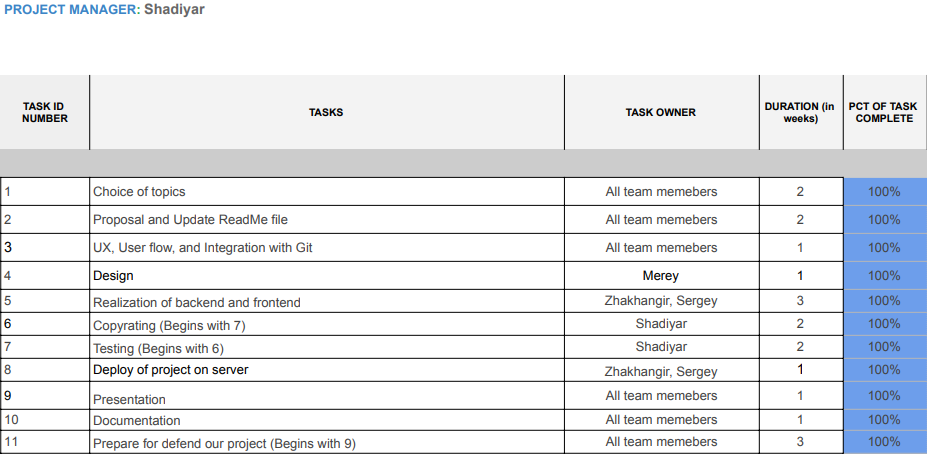
\includegraphics[scale=0.5]{plan1.png}
    \caption{Gantt chart}
    \label{fig:plan1}
\end{figure}

\begin{figure}[ht]
    \centering
    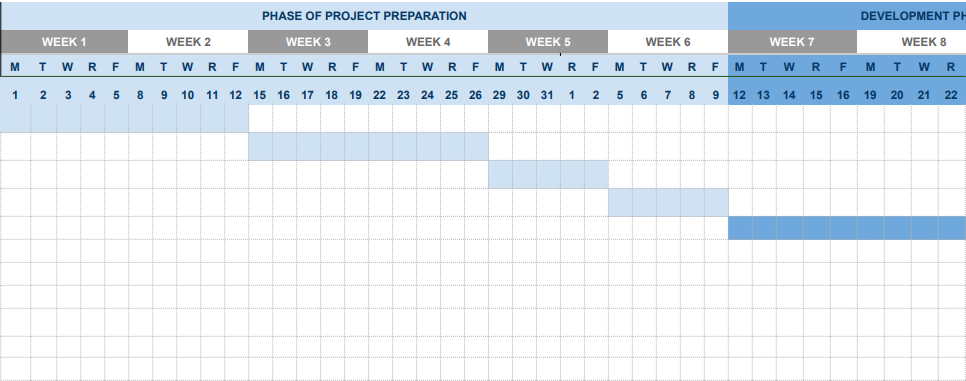
\includegraphics[scale=0.5]{plan2.png}
    \caption{Gantt chart}
    \label{fig:plan2}
\end{figure}

\begin{figure}[ht]
    \centering
    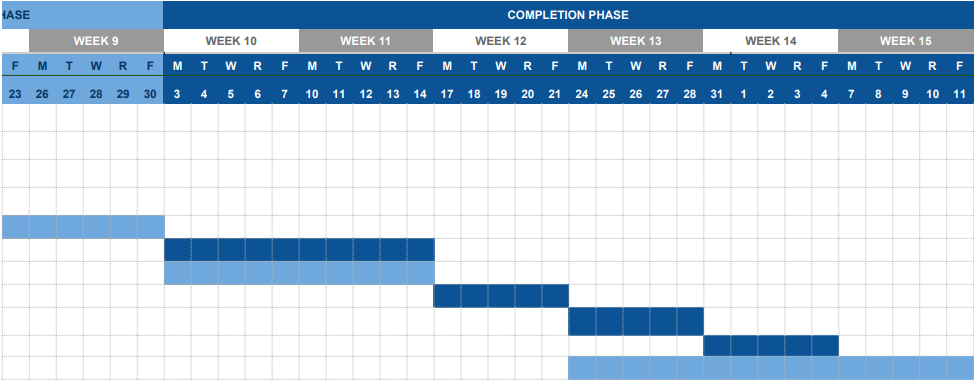
\includegraphics[scale=0.5]{plan3.png}
    \caption{Gantt chart}
    \label{fig:plan3}
\end{figure}

\begin{figure}[ht]
    \centering
    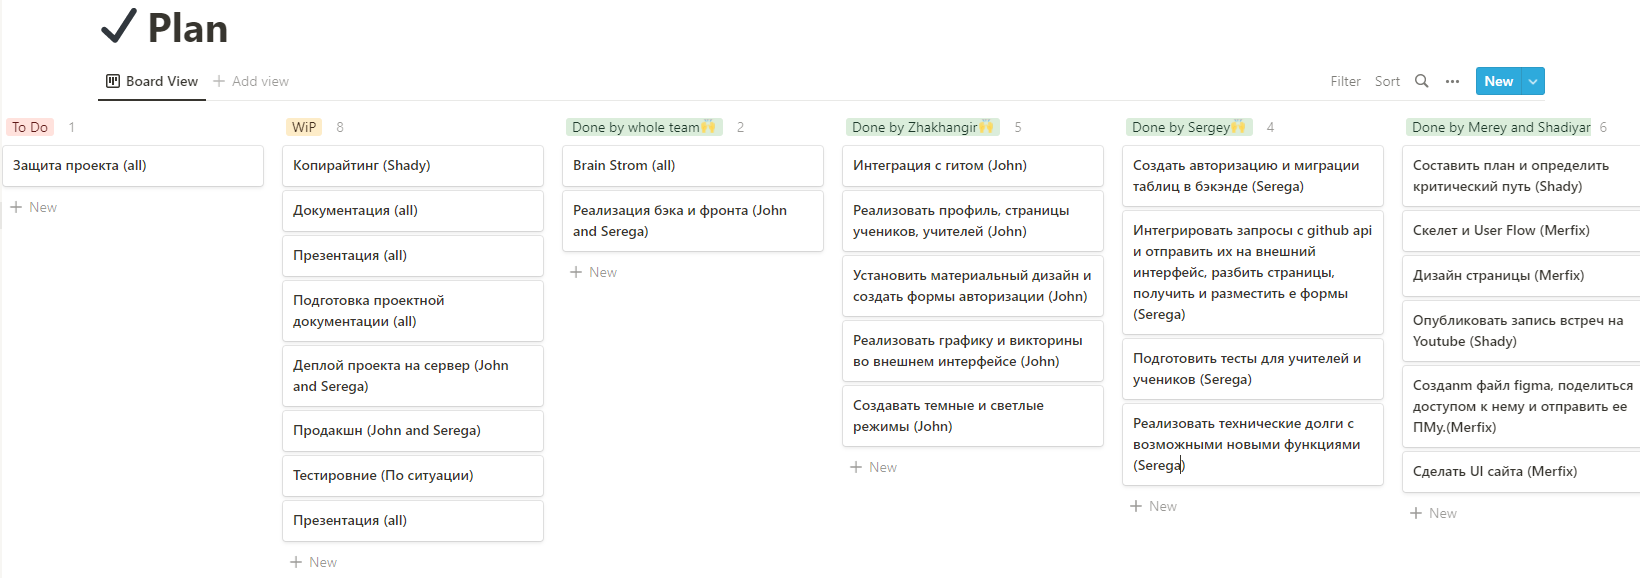
\includegraphics[scale=0.5]{Kanbanbrd.png}
    \caption{Kanban board}
    \label{fig:knbrd}
\end{figure}
%Картинка съезжает, придумать, что с этим делать%
\begin{figure}[t]
    \centering
    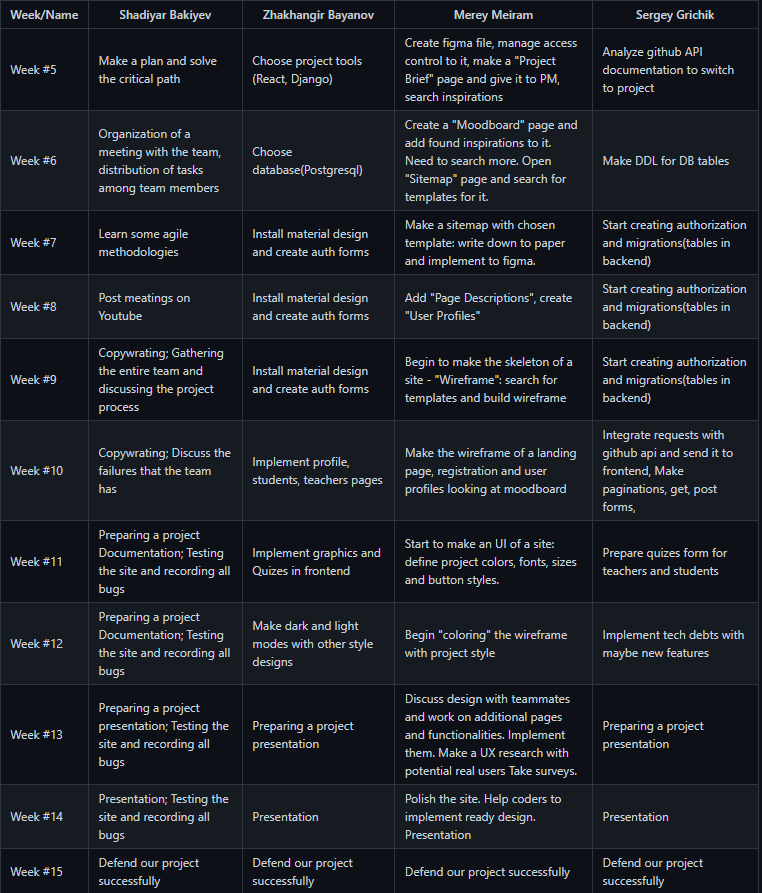
\includegraphics[scale=0.5]{weeksplan.png}
    \caption{Plan on Git}
    \label{fig:weeksplan}
\end{figure}

%\enlargethispage{\baselineskip}
\section{User Personas and Stories}

\section{Sitemap, Page descriptions}

    \chapter{How was the project created?}\label{ch:B}

\section{Project UI}
Stack: postgresql, Django, python, Django ORM. First we structured the DDL diagram for the project database, after that we connected it with django and used the orm system. Most of the logic is the CRUD system. Also there is integration with github api in python where we can reference to their api to send or get some information from user’s githubStack: postgresql, Django, python, Django ORM. First we structured the DDL diagram for the project database, after that we connected it with django and used the orm system. Most of the logic is the CRUD system. Also there is integration with github api in python where we can reference to their api to send or get some information from user’s github %Поменять!!!%
\section{Project Front}
Used mui/material design library for beautiful UI and components respectively. Mui library only used with React js library by Facebook. With React there was used a lot of technologies like Formik, Yup, Lodash etc.
Created centralized components. Example \ref{fig:dgrm}:
\begin{figure}[ht]
    \centering
    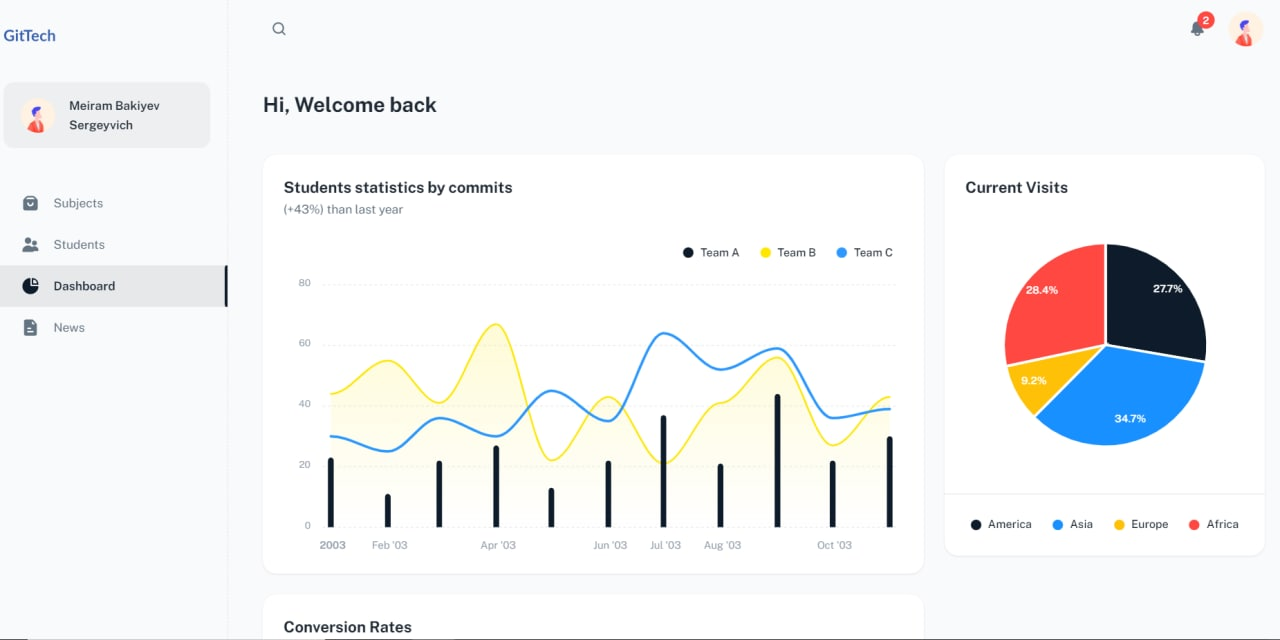
\includegraphics[scale=0.5]{diagramsfnt.jpg}
    \caption{Diagram}
    \label{fig:dgrm}
\end{figure}
Added charts for analytic results, charts like Pie, line. Example \ref{fig:sbj}:
\begin{figure}[ht]
    \centering
    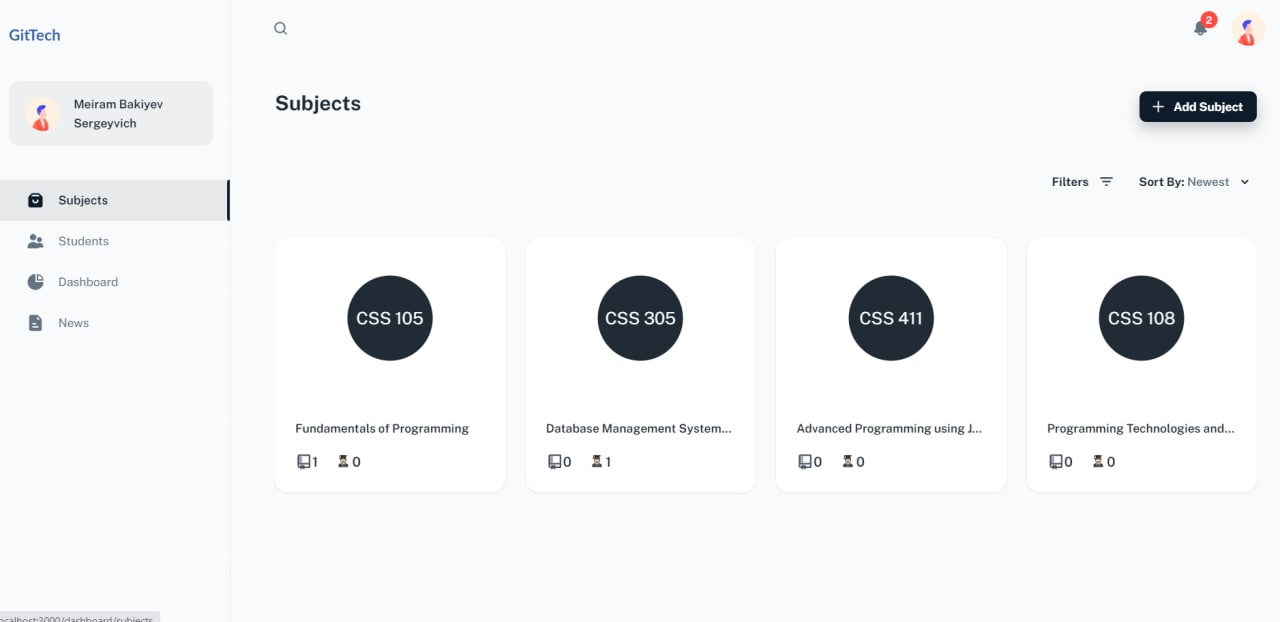
\includegraphics[scale=0.5]{subjectsfnt.jpg}
    \caption{Item selection}
    \label{fig:sbj}
\end{figure}

\section{Project back}
Stack: postgresql, Django, python, Django ORM. First we structured the DDL diagram for the project database, after that we connected it with django and used the orm system. Most of the logic is the CRUD system. Also there is integration with github api in python where we can reference to their api to send or get some information from user’s github
    \chapter{Problems that had to be faced}\label{ch:C}
\section{Problems encountered at the design stage}
\section{Problems encountered at the development stage}
Integration with Github Api was pretty hard to read all documentation here \cite{gitlink} and there was OAuth access token for every request which we send by user, so we solved it by creating new public organization where my own token connected for Github OAuth "accesstoken".


 

    \chapter{Conclusion}\label{ch:concl}
Everything is great, but there is a space for future work.
    
    \appendix
    \chapter{AppendixATitle}\label{app:A}
\section{Theorem}
\section{Proof}
etc. etc.

    \chapter{AppendixBTitle}\label{app:B}
Five little monkeys are jumping on the bed.


    \printbibliography[heading=bibintoc,title={References}]
\end{document}